%!TEX root = ../../terrainbook.tex
% chktex-file 46

\setchapterpreamble[u]{\margintoc}

\graphicspath{{appendices/pcformats/figs/}}

\chapter{Point cloud file formats}%
\label{app:pcformats}


A point cloud is essentially an array of 3D points, and often that is also how it is stored in a file.
Regardless of the format, a point cloud file can often be seen as an array of \emph{point records}, each of which contains the coordinates and potentially some attributes (also called \emph{fields}).

A field stores a single value---\eg\ an integer, a float, or a boolean---and can for instance represent the $x$-, $y$-, or $z$-coordinate of a point or one of its attributes, \eg\ the lidar return number, the classification of the point, or the colour information.
The order and meaning of the fields in a record are usually fixed for all the point records in one file.
\marginnote{$(x,y,z)$ + attributes}
How exactly the point records are structured and stored in the file, and what additional metadata are available, depends on the specific file format that is used.

Notice that, in addition to the widely used formats mentioned here, there are also many proprietary formats. 
These are often specific to one particular software and are therefore not very useful for data exchange.


%%%
%
\section{ASCII formats}

ASCII formats are plain text files\sidenote{\url{https://en.wikipedia.org/wiki/ASCII}}, the point cloud information is thus stored as a sequence of ASCII characters, usually one point record per line.
In most cases you can recognise such files by the \emph{.xyz}, \emph{.csv}, or \emph{.txt} extensions; these are in most cases comma-separated value (CSV) files\sidenote{\url{https://en.wikipedia.org/wiki/Comma-separated_values}}.
A benefit of ASCII files is that you can simply open and edit them in a text editor.
The biggest downside is that they are not standardised, \ie\ the type, order, and number of attributes vary, and also the used coordinate reference system (CRS) is usually not documented in the file.
\begin{figure}
  \begin{verbatim}
    x y z
    84499.948 446610.324 0.407
    84499.890 446609.862 0.434
    84499.832 446609.420 0.442
    84499.777 446608.987 0.454
    84499.715 446608.528 0.444
    84499.839 446612.808 0.493
  \end{verbatim}
  \caption{An example of a CSV file used to store the $xyz$ coordinates of a point cloud. Notice that the delimiter is in this case not a comma but a space.}%
\label{fig:csv}
\end{figure}


%%%
%
\section{PLY format}%
\index{PLY format}

\begin{figure}
  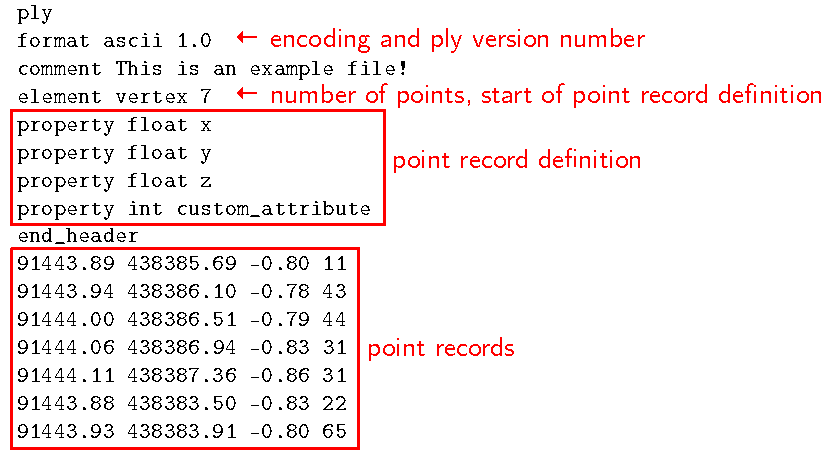
\includegraphics[width=\linewidth]{ply_header.pdf}
  \caption{A simple PLY file with 1 additional user-defined attribute of type integer (\texttt{int}). It contains 7 points.}%
\label{fig:ply}
\end{figure}
The PLY format can be considered a standardised ASCII format.
\marginnote{More information about PLY: \url{http://paulbourke.net/dataformats/ply/}}
A PLY file contains a header\marginnote{A header is supplemental information placed at the beginning of a file, \eg\ to store metadata about the file.} that specifies the structure of the point records in the file, \ie\ the number of attributes (for this format called a \emph{property}), their order, their names, and their data types.
Because the user can decide on the composition of the point record, this makes it a very flexible format.
Figure~\ref{fig:ply} shows an example PLY file.

%

PLY files are readable by many software packages and can also be stored in a binary encoding\marginnote{\url{https://en.wikipedia.org/wiki/PLY_(file_format)\#ASCII_or_binary_format}}.
Compared to the ASCII encoding, the binary encoding results in a smaller file size and quicker reading and writing from and to the file.
There is however no standardised way to specify the CRS in a PLY file, although one could add a comment in the header stating the CRS\@.


%%%
%
\section{LAS format}%
\index{LAS format}


The \emph{LASer} file format (LAS) is the most widely used standard for the dissemination of point cloud data.
The LAS standard, currently at version 1.4\marginnote{LAS v1.4-R15 is the latest version}, is maintained by the American Society for Photogrammetry and Remote Sensing (ASPRS) and, as the name implies, was designed for datasets that originate from (airborne) lidar scanners.
\marginnote{\url{https://github.com/ASPRSorg/LAS}}
However, in practice it is also used for other types of point cloud, \eg\ those derived from dense image matching.
LAS files are binary and unlike the PLY format the fields are prescribed, \ie\ the attributes for each point record are their types (number of bits) cannot be modified.
Table~\ref{tab:las-record} shows the composition of the simplest record type that is available for LAS files.
\begin{table*}
  \centering
  \small
  \begin{tabular}{l|l|r|p{7cm}}
    % \toprule
    % \rowcolor[gray]{.9}
    Field & Format & Length (bits) & Description\\ \midrule
    X & int & 32 & X coordinate \\ 
    Y & int & 32 & Y coordinate \\ 
    Z & int & 32 & Z coordinate \\ 
    Intensity & unsigned int & 16 & The pulse return amplitude \\ 
    Return number & unsigned int & 3 &  The total pulse return number for a given output pulse \\ 
    Number of returns & unsigned int & 3 & Total number of returns for a given pulse \\ 
    Scan Direction Flag & boolean & 1 & Denotes the direction at which the scanner mirror was travelling at the time of the output pulse. A bit value of 1 is a positive scan direction, and a bit value of 0 is a negative scan direction (where positive scan direction is a scan moving from the left side of the in-track direction to the right side and negative the opposite).  \\ 
    Edge of Flight Line & boolean & 1 & Has a value of 1 only when the point is at the end of a scan. It is the last point on a given scan line before it changes direction. \\ 
    Classification & unsigned int & 5 & Classification code \\ 
    Scan Angle Rank & int & 4 & The angle at which the laser pulse was output from the scanner including the roll of the aircraft \\ 
    User Data & unsigned int & 4 & May be used at the user's discretion \\ 
    Point Source ID & unsigned int & 8 & Indicates the file from which this point originated Non-zero if this point was copied from another file
    % \bottomrule
  \end{tabular}
\caption{LAS Point Data Record Format 0}%
\label{tab:las-record}
\end{table*}
In the specifications this is referred to as the ``Format 0'', and other record types are possible (Formats 1 to 10).
Other record types can add for instance the RGB colour information of the point, or the GPS time (the time a point was measured by the scanner), but all records types include at least the fields shown in Table~\ref{tab:las-record}.
While the LAS standard clearly specifies that all these fields are required, some of the fields are very specific to lidar acquisition and they are sometimes ignored in practice, \eg\ if a point cloud originating from dense matching is stored in the LAS format.
\marginnote{Unused fields take up storage} 
It is important to notice that unused fields will still take up storage space in each record (a default value is then assigned, such as 0.0 for floats or 0 for integers).

\paragraph{CRS.}
The CRS of the point cloud can be stored in the header of a LAS file, together with some other general information such as the total number of points and the bounding box of the point cloud. 
The X, Y, and Z fields are stored as 32-bit integers. 
To convert these values to the actual coordinates on the ground, they need to be multiplied by a scaling factor and added to an offset value, \ie:
\begin{gather*}
  X_{coordinate} = (X_{record} * X_{scale}) + X_{offset} \\
  Y_{coordinate} = (Y_{record} * Y_{scale}) + Y_{offset} \\
  Z_{coordinate} = (Z_{record} * Z_{scale}) + Z_{offset}
\end{gather*}
The scaling factors $X_{scale}$, $Y_{scale}$, $Z_{scale}$ and the offsets $X_{offset}$, $Y_{offset}$, $Z_{offset}$ are also listed in the header. 
\marginnote{Scaling factors and offsets are stored in the LAS header}
Notice that the scaling factor determines the number of decimals that can be stored, \eg\ the factors $0.1$, $0.01$, and $0.001$ would give us $1$, $2$, and $3$ decimals respectively.

\paragraph{Classification.}
The LAS standard defines several classification codes, as listed in Table~\ref{tab:las-classes}.
\begin{table}
  \centering
  \begin{tabular}{r|l}
  % \toprule
  % \rowcolor[gray]{.9}
  Code & Meaning \\ \midrule
  0 & never classified \\
  1 & unclassified \\
  2 & ground \\
  3 & low vegetation \\
  4 & medium vegetation \\
  5 & high vegetation \\
  6 & building \\
  7 & low point (noise) \\
  8 & \emph{reserved} \\
  9 & water \\
  13--31 & user-defined \\
  % \bottomrule
\end{tabular}
\caption{The first 10 LAS classification code numbers. More codes exist, but they are not listed here.}%
\label{tab:las-classes}
\end{table}
These codes are to be used as values for the classification field of a point record, and are intended to indicate the type of object a point belongs to.
Which classes are used strongly depends on the dataset at hand.
The codes $0$ and $1$ may appear ambiguous, but there is a clear distinction.
To be exact, the code $0$ is used for points that were never subjected to a classification algorithm, whereas the code $1$ is used for points that have been processed by a classification algorithm, but could not be assigned to a specific class.
It is possible to define your own classes using code ranges that are reserved for that purpose.


%%%
\section{LAZ format}%
\index{LAZ format}

A compressed variant of the LAS format, dubbed ``LAZ'', exists.
\marginnote{\citet{Isenburg13} describes in details the LAS format}
While it is not maintained by an `official' organisation like the LAS standard, it is an open standard and it is widely used, especially for very big dataset.
Through the use of lossless compression algorithms that are specialised for point cloud data, a LAZ file can be compressed into a fraction of the storage space required for the equivalent LAS file, without any loss of information.
This makes it more effective than simply using ZIP compression on a LAS file.
In addition, support for LAZ is typically built into point cloud reading and writing software, so to the user it is no different than opening a LAS file (although the compression and decompression operations do take extra time).

The LAZ format closely resembles the LAS format, \ie\ the header and the structure of the point records are virtually identical.
In a LAZ file the point records are grouped in blocks of 50,000 records each.
\marginnote{LAZ creates blocks of neighbouring points}
Each block is individually compressed, which makes it possible to partially decompress only the needed blocks from a file (instead of always needing to decompress the whole file).
This can save a lot of decompression computations if only a few points from a huge point cloud are needed.
Also notice that the effectiveness of the compression algorithms depends on the similarity in information between subsequent point records.
Typically information is quite similar for points that are close to each other in space.
Therefore, a greater compression factor can often be achieved after spatially sorting the points.

In practice, for the AHN4 dataset, the LAZ file of a given area is about 10X more compact than its LAS counterpart.
\marginnote{LAZ = about 10X compacter than LAS}
However, the main disadvantage is that reading and writing a LAZ file is slower than a LAS file, since more operations need to be performed.

